\section{Arquitectura limpia}\label{sec:clean_architecture}

El uso de una arquitectura limpia en el desarrollo del sistema de extracción de información de documentos asegura que
cada componente del sistema sea independiente y fácil de modificar o reemplazar.
Como veremos, esto permitirá una integración sencilla de nuevas tecnologías y, por lo tanto, la inclusión del soporte
de nuevos tipos de formato o nuevos tipos de documento en el sistema a futuro.

\subsection{Introducción histórica}
En el ámbito del desarrollo de software, la arquitectura de un sistema es crucial para determinar su escalabilidad y
mantenibilidad a largo plazo.

Una de las metodologías que ha cobrado relevancia en este contexto son las ``arquitecturas limpias'', un enfoque para el
diseño de software promovido por Robert C. Martin en su libro Clean Architecture: A Craftsman`s Guide to Software
Structure and Design~\cite{book_martin_2017}.

\subsection{Definición}
La arquitectura limpia es un estilo de diseño que organiza el sistema de manera que sea independiente de los diferentes
elementos a los que considera detalles de implementación y que son intercambiables unos por otros:
\textit{frameworks}, \textit{interfaces}, bases de datos o \textit{API} entre otros.

La esencia de esta arquitectura radica en su diagrama de capas, donde cada capa tiene una responsabilidad claramente
definida y depende solo de las capas más internas.
Esto se logra mediante el principio de inversión de dependencias, lo que significa que los detalles dependen de las
abstracciones y no al contrario.

Existen diferentes implementaciones de ``arquitectura limpia'', cada una con sus características intrínsecas, en este
proyecto hemos decidido implementar la versión en tres capas que aparece en la figura
~\ref{fig:chapter_2.clean_architecture}.

\begin{figure}[ht]
    \begin{center}
        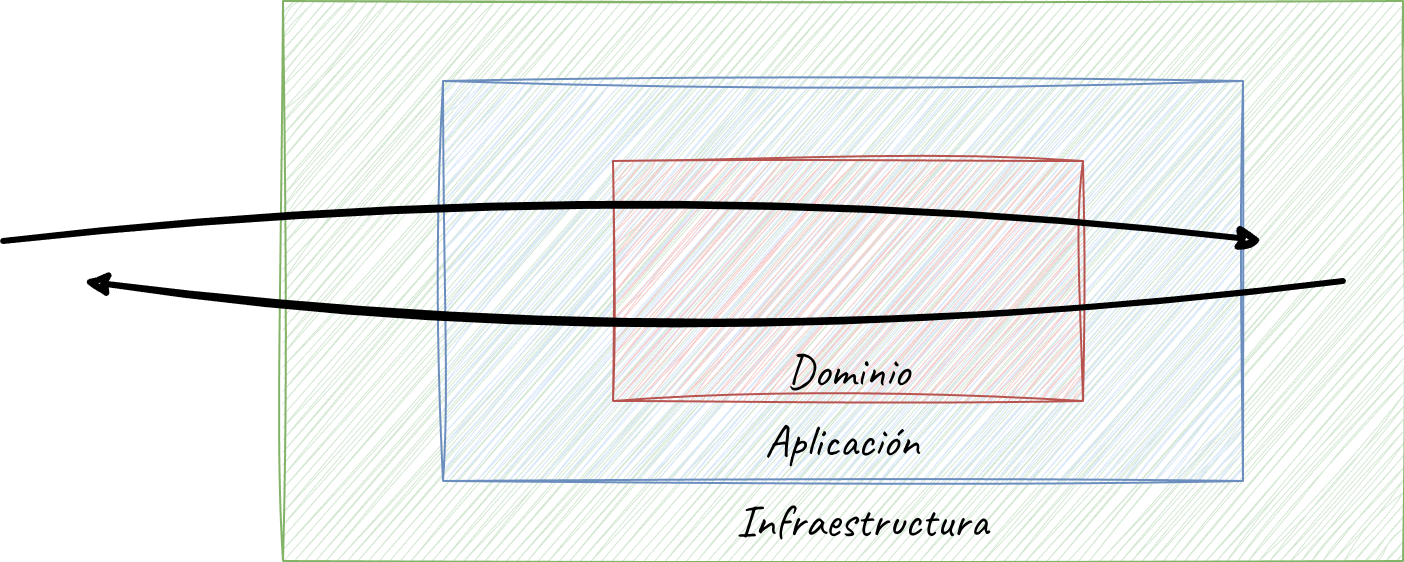
\includegraphics[width=0.5\textwidth]{./chapter/2/images/chapter_2.clean_architecture}
        \caption{Esquema de una arquitectura limpia}
        \label{fig:chapter_2.clean_architecture}
    \end{center}
\end{figure}

La capa más interior se denomina \textbf{capa de dominio} y es el corazón del modelo de negocio de la aplicación y
encapsula la lógica y las reglas del negocio.
Esta capa es fundamentalmente agnóstica respecto a tecnologías externas y se centra exclusivamente en definir los
conceptos fundamentales del negocio.
Algunos de los elementos que puede contener son: entidades, objetos de valor, servicios de dominio, abstracciones

Esta capa debe ser autocontenida y fácilmente testable, aislada de tecnologías externas como bases de datos o
interfaces de usuario.

La capa que aparece a continuación es la \textbf{capa de aplicación}.
La capa de aplicación actúa como un mediador entre la capa exterior y la capa de dominio, coordinando las operaciones
de alto nivel que involucran múltiples aspectos del dominio.

La capa más exterior se denomina \textbf{capa de infraestructura}.
La capa de infraestructura proporciona las capacidades tecnológicas necesarias para que la capa de dominio puedan
realizar sus funciones sin tener que preocuparse por los detalles de implementación.
Toda la comunicación o interacción con elementos externos a la aplicación deben estar contenidos dentro de la capa de
infraestructura.
